\begin{figure*}[t]
  \centering
  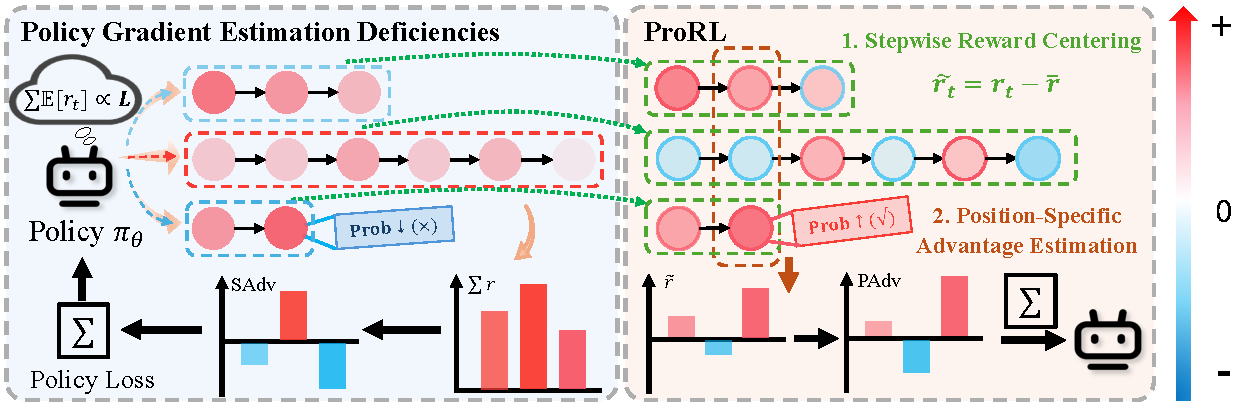
\includegraphics[width=0.9\linewidth]{figure/main_RL_thin.pdf}
  \caption{Overview of our proposed \textbf{ProRL}. (\textbf{Left}) Standard policy gradient estimation suffers from the length shortcut. Since step-level rewards accumulate with positive mean $(\sum_{t=1}^L \mathbb{E}[r_t] \propto L)$, the Sequence-level Advantage~(SAdv) and gradient signal are dominated by length variation, causing the model to extend paths rather than explore diverse alternatives. (\textbf{Right}) ProRL rectifies gradient estimation through two mechanisms. Stepwise Reward Centering ($\tilde{r}_t = r_t - \bar{r}$) ensures that path extension yields zero expected gain. Position-Specific Advantage Estimation (PAdv) computes step-adapted baselines for effective optimization.}
  \label{fig:method}
\end{figure*}

\section{Methodology}
\label{sec:method}
\subsection{Overview}
Section~\ref{sec:analysis} shows that standard policy gradient estimation fails in PRS due to the \emph{length shortcut}: path-level rewards decompose into step-level rewards with positive mean, causing length to dominate the gradient signal. Beyond this, the decomposition structure suggests an opportunity for improvement: standard estimation incurs high gradient variance by weighting each step with the entire path reward, which can be reduced through task-specific adaptation to the per-step reward structure. To address both issues, we propose ProRL with the following two mechanisms, which effectively rectify policy gradient estimation.

\textbf{Stepwise Reward Centering} (Section~\ref{sec:centering}) eliminates the length shortcut: by subtracting the expected reward at each step, we ensure that path extension yields \emph{zero expected gain}, redirecting gradient estimation toward path quality exploration rather than length manipulation.

\textbf{Position-Specific Advantage Estimation} (Section~\ref{sec:advantage}) reduces gradient variance: by computing step-adapted baselines that leverage the decomposition structure of path rewards, we obtain gradient estimates with lower variance. 

Together, these rectifications yield policy gradient estimation that achieves effective RL for PRS. Figure~\ref{fig:method} illustrates the complete framework.

\subsection{Stepwise Reward Centering}
\label{sec:centering}

By Eq.~\eqref{eq:reward_decomposition}, path-level rewards in PRS decompose as $R = \sum_{t=1}^{L} r_t$, where step-level rewards $r_t$ exhibit positive mean $\mathbb{E}_\pi[r_t]$. This couples expected return with path length, causing the length shortcut. Our design is to break this coupling: \emph{path extension should yield zero expected gain}.

We achieve this through reward centering. Empirically, we observe that $\mathbb{E}_{\pi}[r_t]$ remains relatively stable for many rewards (e.g., IoI; see Figure~\ref{fig:length-collapse}). For simplicity, we use a single global statistic $\bar{r}$ rather than 
step-specific estimates. We define the centered reward as: 
\begin{equation}
\tilde{r}_t = r_t - \bar{r}, \quad \text{where} \quad \bar{r} = \mathbb{E}_{\pi}\left[r_*\right].
\label{eq:centering}
\end{equation}
Here $\bar{r}$ is the global expected step reward, where the subscript ``$*$'' denotes any step. By construction, $\mathbb{E}_{\pi}[\tilde{r}_t] = 0$ for all $t$. Therefore, $\mathbb{E}\left[\sum_{t=1}^{L} \tilde{r}_t\right]$ is independent on path length $L$. The length shortcut is eliminated: the model cannot improve rewards by extending paths, and must instead explore deeply into path quality. In practice, we estimate $\bar{r}$ via online accumulation over rollouts of the first training epoch and freeze it for all subsequent epochs. We discuss alternatives to eliminating the length shortcut in Appendix~\ref{app:alternatives}.

\paragraph{Multi-Objective Reward.} Path quality in PRS involves multiple objectives. To handle this, suppose we have $K$ separate path-level rewards $\{R^{(i)}\}_{i=1}^{K}$, each decomposing into step-level rewards $R^{(i)}=\sum_t r_t^{(i)}$. Since these components have different scales, we extend \emph{centering} to \emph{normalization}:
\begin{equation}
\tilde{r}_t = \sum_{i=1}^{K} w_i \cdot \frac{r_t^{(i)} - \mu^{(i)}}{\sigma^{(i)}},
\label{eq:reward-normalize}
\end{equation}
where $\mu^{(i)} = \mathbb{E}_{\pi}\left[r_*^{(i)}\right]$ and $\sigma^{(i)} = \sqrt{\mathrm{Var}_{\pi}\left(r_*^{(i)}\right)}$ are estimated from rollouts during a warm-up epoch, avoiding the drift that would otherwise arise from co-evolving $\mu, \sigma$ and $\pi$ as the policy improves. The resulting normalization centers each component and rescales them to comparable magnitudes, enabling multi-objective optimization.

\subsection{Position-Specific Advantage Estimation}
\label{sec:advantage}

Stepwise Reward Centering eliminates the length shortcut, but effective training also requires low-variance gradient estimates. Recall from Section~\ref{sec:task} that the standard gradient estimator $\hat{g}_{\mathrm{std}}$ (Eq.~\eqref{eq:g-std}) weights each step's gradient by the total path reward $R^{(i,j)}$. However, the item at step $t$ only affects rewards from $t$ onward; including earlier rewards $r_1, \ldots, r_{t-1}$ introduces irrelevant noise.

We leverage the structural property that path-level rewards decompose into step-level rewards. For step $t$, we define the \emph{reward-to-go} $G_t^{(i,j)} = \sum_{\ell=t}^{L^{(i, j)}} r_\ell^{(i,j)}$ as the cumulative reward from $t$ onward. Replacing $R^{(i,j)}$ with $G_t^{(i,j)}$ excludes past rewards unaffected by the current action:
\begin{equation}
\hat{g}_{\mathrm{rtg}} = \frac{1}{nm}\sum_{i=1}^{n}\sum_{j=1}^{m}\left[\sum_{t=1}^{L^{(i,j)}} \nabla_\theta \log \pi_\theta^{(i,j,t)} \cdot G_t^{(i,j)}\right].
\label{eq:g-rtg}
\end{equation}
Variance can be reduced further by centering $G_t$ around its expected value. According to classical RL results~\cite{Williams92simple}, subtracting a baseline from the reward-to-go yields an \emph{advantage}, which is an unbiased and lower-variance estimate that measures relative quality rather than absolute return. Traditionally, this requires training an auxiliary critic model, adding complexity and computational cost.

Recent work on LLM alignment, notably GRPO~\cite{shao2024deepseekmath}, avoids the critic by using group Monte Carlo estimation: the baseline is simply the mean path reward across rollouts from the same input, $\bar{R}_i = \frac{1}{m}\sum_{j=1}^m R^{(i,j)}$. However, this path-level baseline is shared across all steps, ignoring that the expected reward-to-go varies by position.

Inspired by GRPO, we use the per-step reward structure of PRS to compute \emph{position-specific baseline} $\bar{G}_{i,t}$, the average reward-to-go at step $t$ across all paths from the $i$-th input that reach step $t$. The \emph{position-specific advantage} is then:
\begin{equation}
\bar{G}_{i,t} = \frac{\sum_{j: L^{(i,j)} \geq t} G_t^{(i,j)}}{\sum_{j=1}^{m} \mathbb{I}[L^{(i,j)} \geq t]}, \quad \hat{A}_t^{(i,j)} = G_t^{(i,j)} - \bar{G}_{i,t}.
\label{eq:step-advantage}
\end{equation}
Unlike GRPO's uniform baseline, each step $t$ has its own reference point $\bar{G}_{i,t}$, adapting to the expected future return at that position. Our rectified gradient estimator is:
\begin{equation}
\hat{g}_{\mathrm{rect}} = \frac{1}{nm}\sum_{i=1}^{n}\sum_{j=1}^{m}\left[\sum_{t=1}^{L^{(i,j)}} \nabla_\theta \log \pi_\theta^{(i,j,t)} \cdot \hat{A}_t^{(i,j)}\right].
\label{eq:g-rect}
\end{equation}
This design reduces variance via two well-established mechanisms from 
classical policy gradient literature~\citep{Williams92simple,sutton1999policy}. 
First, reward-to-go excludes past rewards $r_1, \ldots, r_{t-1}$ that are unaffected by the action at step $t$, removing irrelevant noise from the gradient signal. Second, the position-specific baseline $\bar{G}_{i,t}$ adapts to the expected future return at each position, providing a tighter reference than a path-level baseline. Both techniques are known to preserve unbiasedness while reducing gradient variance~\citep{GreensmithBB01}. Ablation study (Section~\ref{sec:ablation_gradient}) 
empirically validates the effectiveness of $\hat{g}_{\mathrm{rect}}$.